\section{Results}

Put results of playing around with service mesh here...

\begin{itemize}
	\item it's abit more than \linkerd{}.
	\item We will need to know about \lstinline|kubectl|.
\end{itemize}

\subsection{Showcases Implementation}
This is what the showcases called in \autoref{sec:showcases-1} look like with \linkerd{}.

\subsubsection{Encryption}
From the second that a service is injected by \linkerd{} and applied to the cluster, all communication to that service is automatically encrypted.
This holds not only for our self-implemented communication but also for metrics- and tap-services.
Since the communication is proxied by \linkerd{} it activates certificate distribution and encryption out of box.

If you don't want to use this feature, you can disable by overwriting the \linkerd{} configuration.
The following command will generate an updated YAML-configuration you can apply in Kubernetes.
\begin{lstlisting}
linkerd install \
  --disable-identity \
  --disable-tap
\end{lstlisting}
Note: Once this configuration is applied, the will be neither encryption in communication between services nor in tap- and metrics-services.

\subsubsection{Canary Deployment}
\label{sec:canary-result}
TBD

-new service called \lstinline|nameapi-v2|

-doing the same but printing the surname also.

\begin{lstlisting}
apiVersion: split.smi-spec.io/v1alpha1
kind: TrafficSplit
metadata:
	name: nameapi-split
	namespace: default
spec:
	service: nameapi
	backends:
	- service: nameapi
		weight: 90
	- service: nameapi-v2
		weight: 10
\end{lstlisting}


\autoref{fig:results-traffic-split-tree}

\begin{figure}
	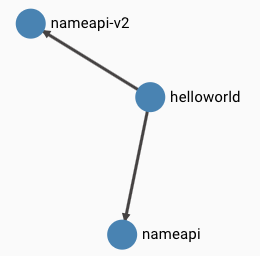
\includegraphics[width=.5\columnwidth]{img/results-traffic-split-tree}
	\centering
	\caption{Delegation tree of \textsc{hello-world-service} after traffic split 90/10.}
	\label{fig:results-traffic-split-tree}
\end{figure}


\autoref{fig:results-traffic-split-weights}

\begin{figure}
	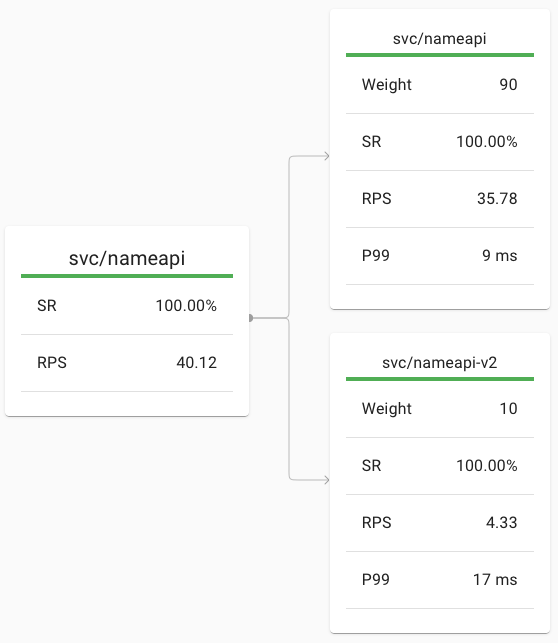
\includegraphics[width=\columnwidth]{img/results-traffic-split-weights}
	\caption{\linkerd{} displays the weights of the 90/10 traffic split.}
	\label{fig:results-traffic-split-weights}
\end{figure}


\subsubsection{Access Policies}
TBD

\subsubsection{Load Balancing}
\label{sec:load-result}

In the \lstinline|spec:|-section setting the count of replicas up to 3 (\lstinline|replicas: 3|).

\autoref{fig:results-load-balance}

\begin{figure}
	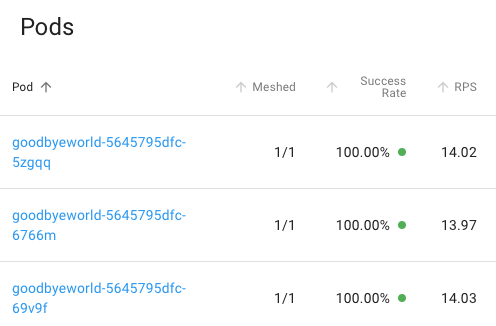
\includegraphics[width=\columnwidth]{img/results-load-balance}
	\caption{The \textsc{goodbye-world-service} deployment shows all three replicas balancing the request-load.}
	\label{fig:results-load-balance}
\end{figure}

TBD
\begin{itemize}
	\item integrated in \linkerd{}
	\item if ingress is "injected", honor;)
\end{itemize}

\subsubsection{Central Monitoring and Logging}
\begin{itemize}
	\item Monitoring comes "out-of-box"
	\item as it was shown in images in \autoref{sec:canary-result} and \autoref{sec:load-result}
	\begin{itemize}
		\item \linkerd{} brings \textsc{Prometheus} and \textsc{Grafana}
		\item  Now we can see \textbf{who} is talking \textbf{how much} to \textbf{whom}
		\item Maybe show a call-tree from linkerd-dashboard?
	\end{itemize}

	\item Logging (\lstinline|linkerd logs|) by linkerd was removed, since it was the same as logs from \lstinline|kubectl|\\
	(\url{https://github.com/linkerd/linkerd2/discussions/5790})
	\item How to use \lstinline|kubectl|?\\
		\lstinline|kubectl logs <pod> <service>|
	\item here the \lstinline|bash-completion| is very useful (see appendix)
	\item often read: \textsc{Loki} as logging solution...?
	\begin{itemize}
		\item easy to embed into  Grafana
	\end{itemize}
\end{itemize}


\subsection{Pitfalls}
...and lessons learned?
\begin{itemize}
	\item \linkerd{} says, it'll need only 2GB of RAM 
	\begin{itemize}
		\item that was not enough. K8s was crashing
		\item With 4 GB it works
	\end{itemize}

	\item Minikube
	\begin{itemize}
		\item use command to build docker images into minikube-environment to be available in K8s.
	\end{itemize}

	\item Bring some time...
	\item use bash-completion
	\item Use ssh-port-forwarding to communicate with dashboard on VPS	
\end{itemize}

For further details on the setup, configuration and usage, see the appendix.